\documentclass[gmd, manuscript]{copernicus} % uncomment to see what the 2 column final paper will look like.

\begin{document}

\section{The emulator}

We treat the output of the simulator $y$ as an uncertain function $f()$ of the simulator inputs $x$, so that $y = f(x)$. We wish to produce a predictive distribution for $y$ at any model input, conditional on the points already run, or the design $(Y, X)$. Throughout the study, we use a kriging function, similar to a Gaussian process regression emulator, as coded in the package DiceKriging \citep{roustant2012dicekriging} in the statistical programming environment R \citep{Rcore2016}, for prediction of climate simulator output at untried inputs.
The kriging model or Gaussian Process regression is specified hierarchically with a separate mean and covariance function. For prediction purposes, \emph{a priori} assume that the trend is a simple linear function of the inputs, and adjust with a Gaussian process. 

%\begin{equation}
$$
f(x) = h(x)^T \beta + Z(x)
$$
%\end{equation}

Where $h(x)^T \beta$ is the mean function, and the residual process $Z$ is a zero mean stationary Gaussian process. The covariance kernel $c$ of $Z$ 

$$
Cov(Z, Z') = \sigma^2 c(x,x')
$$
can be specified in a number of different ways: we use the default diceKriging option of a Matern $v=5/2$ function so that

$$
c(x,x') = (1 + \frac{\sqrt{5} | x - x'|}{\theta} + \frac{5 | x - x'|^2}{3 \theta^2})exp(- \frac{\sqrt{5} |x-x'|}{\theta})
$$

where $\theta$ describes the \emph{characteristic length scales} - a measure of how quickly information about the function is lost moving away from a design point, in any dimension. This and other hyperparameters are estimated via maximum likelihood estimation from the design $(Y, X)$, meaning that the approach is not fully Bayesian (such an approach would find posterior distributions for the hyperparameters rather than point estimates). We use Universal Kriging, with no `nugget' term, meaning that the uncertainty on model outputs shrinks to zero at the design points. 

Full details of the Universal kriging process used can be found in \citep{roustant2012dicekriging}, section 2.1, details of the kernel can be found in section 2.3, and examples of the trend and hyperparameter estimation  in section 3 the same publication. 

\section{Forest regions}

Forest fraction data is taken by calculating the mean broadleaf forest fraction in the areas shown in figure \ref{fig:map_forests}. Mean temperature and precipitation from the model are calculated for the corresponding regions and time period. The regions are: Amazon 15\textdegree S - 15\textdegree N, 270\textdegree E - 315\textdegree E; Central Africa; 15\textdegree S - 10\textdegree N, 7.5\textdegree E - 30\textdegree E; SE Asia 12\textdegree S - 10\textdegree N, 90\textdegree E - 150\textdegree E.

\begin{figure}[t]
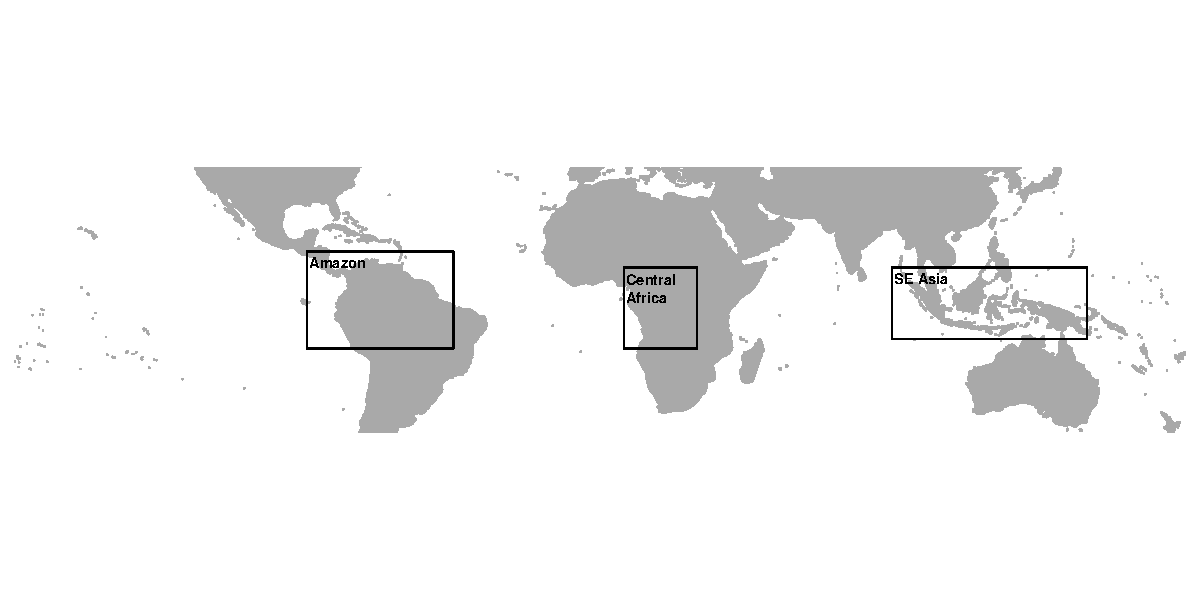
\includegraphics[width=12cm]{../graphics/map_forests_augmented.pdf}
\caption{A map of the forest regions used in the study. }
\label{fig:map_forests}
\end{figure}



\bibliographystyle{copernicus}
\bibliography{augmented.bib}







\end{document}